\documentclass[sigconf]{acmart}

\usepackage{booktabs} % For formal tables
\usepackage{graphicx}
\usepackage{rotating}
\definecolor{Gray}{gray}{0.6}
\usepackage{xspace}

% Copyright
%\setcopyright{none}
%\setcopyright{acmcopyright}
%\setcopyright{acmlicensed}
\setcopyright{rightsretained}
%\setcopyright{usgov}
%\setcopyright{usgovmixed}
%\setcopyright{cagov}
%\setcopyright{cagovmixed}


% DOI
\acmDOI{10.475/123_4}

% ISBN
\acmISBN{123-4567-24-567/08/06}

%Conference
\acmConference[GECCO '17]{the Genetic and Evolutionary Computation Conference 2017}{July 15--19, 2017}{Berlin, Germany}
\acmYear{2017}
\copyrightyear{2017}

\acmPrice{15.00}



%%%%%%%%%%%%%%%%%%%%%%   END OF PREAMBLE   %%%%%%%%%%%%%%%%%%%%%%%%%%%%%%%%%%%%

%%%%%%%%%%%%%%%%%%%%%%%%%%%%%%%%%%%%%%%%%%%%%%%%%%%%%%%%%%%%%%%%%%%%%%%%%%%%%%%
%%%%%%%%% TO BE EDITED %%%%%%%%%%%%%%%%%%%%%%%%%%%%%%%%%%%%%%%%%%%%%%%%%%%%%%%%
%%%%%%%%%%%%%%%%%%%%%%%%%%%%%%%%%%%%%%%%%%%%%%%%%%%%%%%%%%%%%%%%%%%%%%%%%%%%%%%
% rungeneric.py writes data into a subfolder of ppdata
\newcommand{\bbobdatapath}{ppdata/} % change default output folder of COCO if desired
\input{\bbobdatapath cocopp_commands.tex} % provide default of algname and algfolder
% \renewcommand{\algname}{MYNAME}  % name of algorithm as it should appear in the text
% \renewcommand{\algfolder}{ABC/} % subfolder of \bbobdatapath for processed algorithm
%%%%%%%%%%%%%%%%%%%%%%%%%%%%%%%%%%%%%%%%%%%%%%%%%%%%%%%%%%%%%%%%%%%%%%%%%%%%%%%
%%%%%%%%%%%%%%%%%%%%%%%%%%%%%%%%%%%%%%%%%%%%%%%%%%%%%%%%%%%%%%%%%%%%%%%%%%%%%%%
%%%%%%%%%%%%%%%%%%%%%%%%%%%%%%%%%%%%%%%%%%%%%%%%%%%%%%%%%%%%%%%%%%%%%%%%%%%%%%%
\graphicspath{{\bbobdatapath\algfolder}}

\newcommand{\DIM}{\ensuremath{\mathrm{DIM}}}
\newcommand{\aRT}{\ensuremath{\mathrm{aRT}}}
\newcommand{\FEvals}{\ensuremath{\mathrm{FEvals}}}
\newcommand{\nruns}{\ensuremath{\mathrm{Nruns}}}
\newcommand{\Dfb}{\ensuremath{\Delta f_{\mathrm{best}}}}
%\newcommand{\Df}{\ensuremath{\Delta f}}
\newcommand{\DI}{\ensuremath{\Delta I_{\mathrm{HV}}^{\mathrm{COCO}}}}
\newcommand{\nbFEs}{\ensuremath{\mathrm{\#FEs}}}
\newcommand{\ftarget}{\ensuremath{f_\mathrm{t}}}
\newcommand{\CrE}{\ensuremath{\mathrm{CrE}}}
\newcommand{\hvref}{\ensuremath{I_\mathrm{ref}}}
\newcommand{\fopt}{\hvref}
\newcommand{\change}[1]{{\color{red} #1}}
\newcommand{\TODO}[1]{{\color{orange} !!! #1 !!!}}
\newcommand{\bbobbiobj}{{\ttfamily bbob-biobj}\xspace}

%%%%%%%%%%%%%%%%%%%%%%   END OF PREAMBLE   %%%%%%%%%%%%%%%%%%%%%%%%%%%%%%%%%%%%

\begin{document}


\title{Black-Box Optimization Benchmarking Template for the Bi-Objective \bbobbiobj Test Suite}
\renewcommand{\shorttitle}{Template for Benchmarking Single Algorithms on the \bbobbiobj Testbed}
\titlenote{Submission deadline: March 31st.}
%Camera-ready paper due April 24th.}}
\subtitle{Draft version}



\author{Firstname Lastname}
%\authornote{tba if needed}
%\orcid{1234-5678-9012}
%\affiliation{%
%  \institution{Institute for Clarity in Documentation}
%  \streetaddress{P.O. Box 1212}
%  \city{Dublin} 
%  \state{Ohio} 
%  \postcode{43017-6221}
%}
%\email{trovato@corporation.com}
%
%\author{G.K.M. Tobin}
%\authornote{The secretary disavows any knowledge of this author's actions.}
%\affiliation{%
%  \institution{Institute for Clarity in Documentation}
%  \streetaddress{P.O. Box 1212}
%  \city{Dublin} 
%  \state{Ohio} 
%  \postcode{43017-6221}
%}
%\email{webmaster@marysville-ohio.com}
%
%\author{Lars Th{\o}rv{\"a}ld}
%\authornote{This author is the
%  one who did all the really hard work.}
%\affiliation{%
%  \institution{The Th{\o}rv{\"a}ld Group}
%  \streetaddress{1 Th{\o}rv{\"a}ld Circle}
%  \city{Hekla} 
%  \country{Iceland}}
%\email{larst@affiliation.org}
%
%\author{Lawrence P. Leipuner}
%\affiliation{
%  \institution{Brookhaven Laboratories}
%  \streetaddress{P.O. Box 5000}}
%\email{lleipuner@researchlabs.org}
%
%\author{Sean Fogarty}
%\affiliation{%
%  \institution{NASA Ames Research Center}
%  \city{Moffett Field}
%  \state{California} 
%  \postcode{94035}}
%\email{fogartys@amesres.org}
%
%\author{Charles Palmer}
%\affiliation{%
%  \institution{Palmer Research Laboratories}
%  \streetaddress{8600 Datapoint Drive}
%  \city{San Antonio}
%  \state{Texas} 
%  \postcode{78229}}
%\email{cpalmer@prl.com}
%
%\author{John Smith}
%\affiliation{\institution{The Th{\o}rv{\"a}ld Group}}
%\email{jsmith@affiliation.org}
%
%\author{Julius P.~Kumquat}
%\affiliation{\institution{The Kumquat Consortium}}
%\email{jpkumquat@consortium.net}

% The default list of authors is too long for headers}
\renewcommand{\shortauthors}{Firstname Lastname et. al.}


\begin{abstract}
to be written
\end{abstract}


%
% The code below should be generated by the tool at
% http://dl.acm.org/ccs.cfm
% Please copy and paste the code instead of the example below. 
%
 \begin{CCSXML}
<ccs2012>
<concept>
<concept_id>10010147.10010178.10010205.10010208</concept_id>
<concept_desc>Computing methodologies~Continuous space search</concept_desc>
<concept_significance>500</concept_significance>
</concept>
</ccs2012>
\end{CCSXML}

\ccsdesc[500]{Computing methodologies~Continuous space search}


% We no longer use \terms command
%\terms{Algorithms}

% Complete with anything that is needed
\keywords{Benchmarking, Black-box optimization, Bi-objective optimization}

\maketitle


% \section{Introduction}
%
% \section{Algorithm Presentation}
%
% \section{Experimental Procedure}
% \subsection{Parameter Tuning}
%
%%%%%%%%%%%%%%%%%%%%%%%%%%%%%%%%%%%%%%%%%%%%%%%%%%%%%%%%%%%%%%%%%%%%%%%%%%%%%%%
\section{CPU Timing}
%%%%%%%%%%%%%%%%%%%%%%%%%%%%%%%%%%%%%%%%%%%%%%%%%%%%%%%%%%%%%%%%%%%%%%%%%%%%%%%
% note that the following text is just a proposal and can/should be changed to your needs:
In order to evaluate the CPU timing of the algorithm, we have run the \change{\algname} with restarts on the entire bbob-biobj test suite \cite{biobj2016func} for $2 D$ function evaluations according to \cite{hansen2016exp}. The \change{C/Java/Matlab/Octave/Python} code was run on a \change{Mac Intel(R) Core(TM) i5-2400S CPU @ 2.50GHz} with \change{1} processor and \change{4} cores \change{and (compile) options xxx}. The time per function evaluation for dimensions 2, 3, 5, 10, 20\change{, 40} equals \change{$x.x$}, \change{$x.x$}, \change{$x.x$}, \change{$xx$}, \change{$xxx$}\change{, and $xxx$} seconds respectively. 


%%%%%%%%%%%%%%%%%%%%%%%%%%%%%%%%%%%%%%%%%%%%%%%%%%%%%%%%%%%%%%%%%%%%%%%%%%%%%%%
\section{Results}
%%%%%%%%%%%%%%%%%%%%%%%%%%%%%%%%%%%%%%%%%%%%%%%%%%%%%%%%%%%%%%%%%%%%%%%%%%%%%%%

Results of \algname\ from experiments according to \cite{hansen2016exp}, \cite{hansen2016perfass} and \cite{biobj2016perfass} on the benchmark
functions given in \cite{biobj2016func} are presented in
Figures~\ref{fig:ECDFsingleOne}, \ref{fig:ECDFsingleTwo}, \ref{fig:ECDFsingleThree}, and \ref{fig:ECDFsGroups}, and in
Tables~\ref{tab:aRTs5} and \ref{tab:aRTs20}. The experiments were performed with COCO \cite{hansen2016cocoplat}, version \change{2.0}, the plots were produced with version \change{2.0}.

%%%%%%%%%%%%%%%%%%%%%%%%%%%%%%%%%%%%%%%%%%%%%%%%%%%%%%%%%%%%%%%%%%%%%%%%%%%%%%%
%%%%%%%%%%%%%%%%%%%%%%%%%%%%%%%%%%%%%%%%%%%%%%%%%%%%%%%%%%%%%%%%%%%%%%%%%%%%%%%

% Scaling of ECDFs with dimension

%%%%%%%%%%%%%%%%%%%%%%%%%%%%%%%%%%%%%%%%%%%%%%%%%%%%%%%%%%%%%%%%%%%%%%%%%%%%%%%
\begin{figure*}
\centering
\begin{tabular}{@{\hspace*{-0.018\textwidth}}l@{\hspace*{-0.02\textwidth}}l@{\hspace*{-0.02\textwidth}}l@{\hspace*{-0.02\textwidth}}l@{\hspace*{-0.02\textwidth}}}
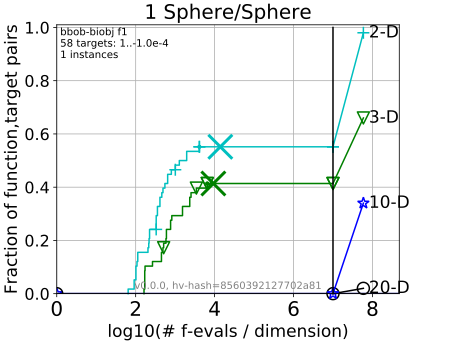
\includegraphics[width=0.25\textwidth]{pprldmany-single-functions/pprldmany_f001}&
\includegraphics[width=0.25\textwidth]{pprldmany-single-functions/pprldmany_f002}&
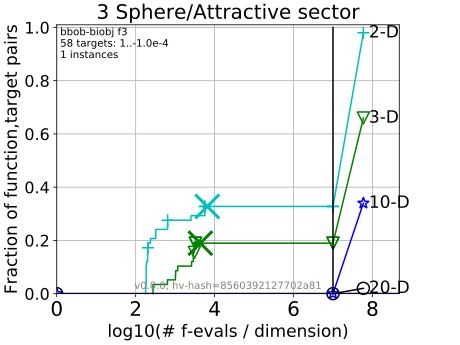
\includegraphics[width=0.25\textwidth]{pprldmany-single-functions/pprldmany_f003}&
\includegraphics[width=0.25\textwidth]{pprldmany-single-functions/pprldmany_f004}\\
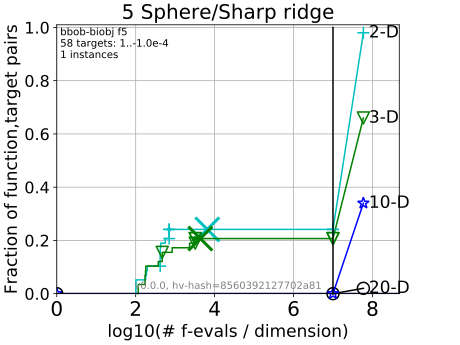
\includegraphics[width=0.25\textwidth]{pprldmany-single-functions/pprldmany_f005}&
\includegraphics[width=0.25\textwidth]{pprldmany-single-functions/pprldmany_f006}&
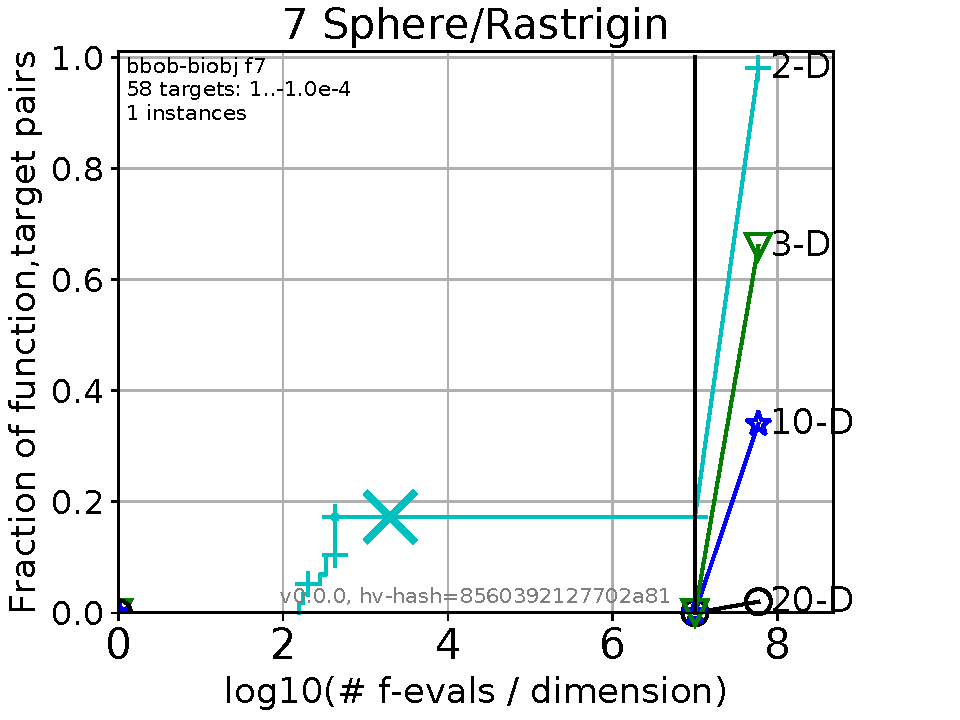
\includegraphics[width=0.25\textwidth]{pprldmany-single-functions/pprldmany_f007}&
\includegraphics[width=0.25\textwidth]{pprldmany-single-functions/pprldmany_f008}\\
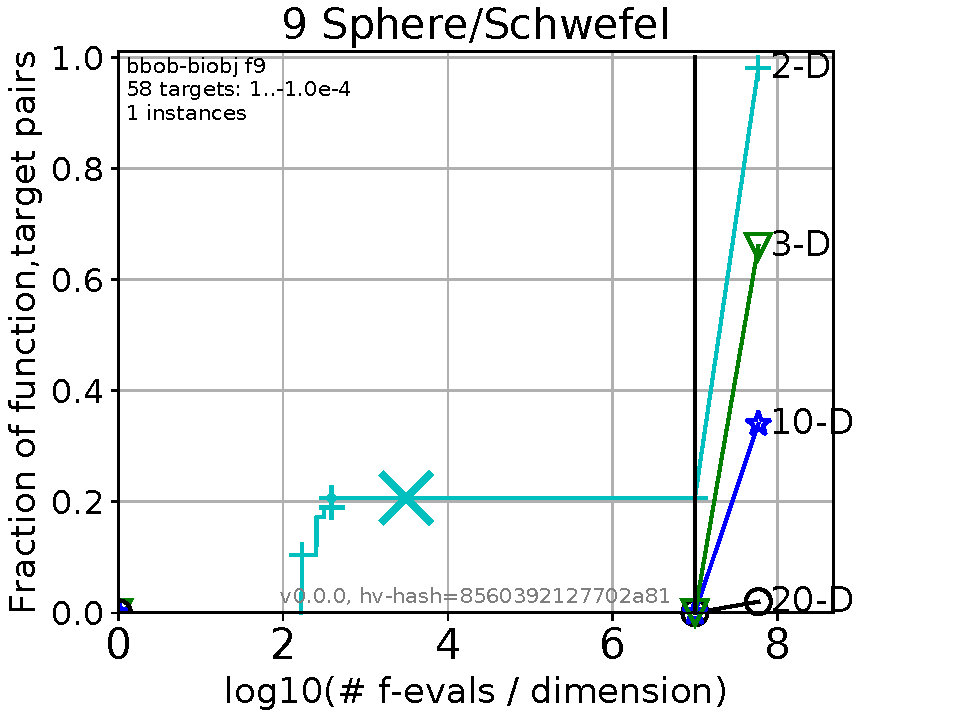
\includegraphics[width=0.25\textwidth]{pprldmany-single-functions/pprldmany_f009}&
\includegraphics[width=0.25\textwidth]{pprldmany-single-functions/pprldmany_f010}&
\includegraphics[width=0.25\textwidth]{pprldmany-single-functions/pprldmany_f011}&
\includegraphics[width=0.25\textwidth]{pprldmany-single-functions/pprldmany_f012}\\
\includegraphics[width=0.25\textwidth]{pprldmany-single-functions/pprldmany_f013}&
\includegraphics[width=0.25\textwidth]{pprldmany-single-functions/pprldmany_f014}&
\includegraphics[width=0.25\textwidth]{pprldmany-single-functions/pprldmany_f015}&
\includegraphics[width=0.25\textwidth]{pprldmany-single-functions/pprldmany_f016}\\[-1.8ex]
\end{tabular}
 \caption{\label{fig:ECDFsingleOne}
 \bbobecdfcaptionsinglefcts{1}{16}
}

\end{figure*}
\begin{figure*}
\centering
\begin{tabular}{@{\hspace*{-0.018\textwidth}}l@{\hspace*{-0.02\textwidth}}l@{\hspace*{-0.02\textwidth}}l@{\hspace*{-0.02\textwidth}}l@{\hspace*{-0.02\textwidth}}l@{\hspace*{-0.02\textwidth}}}
\includegraphics[width=0.25\textwidth]{pprldmany-single-functions/pprldmany_f017}&
\includegraphics[width=0.25\textwidth]{pprldmany-single-functions/pprldmany_f018}&
\includegraphics[width=0.25\textwidth]{pprldmany-single-functions/pprldmany_f019}&
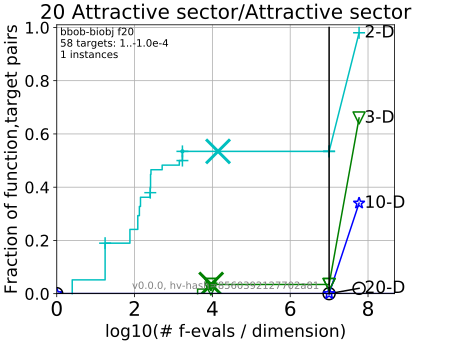
\includegraphics[width=0.25\textwidth]{pprldmany-single-functions/pprldmany_f020}\\
\includegraphics[width=0.25\textwidth]{pprldmany-single-functions/pprldmany_f021}&
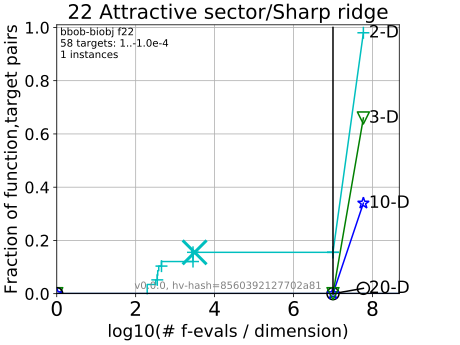
\includegraphics[width=0.25\textwidth]{pprldmany-single-functions/pprldmany_f022}&
\includegraphics[width=0.25\textwidth]{pprldmany-single-functions/pprldmany_f023}&
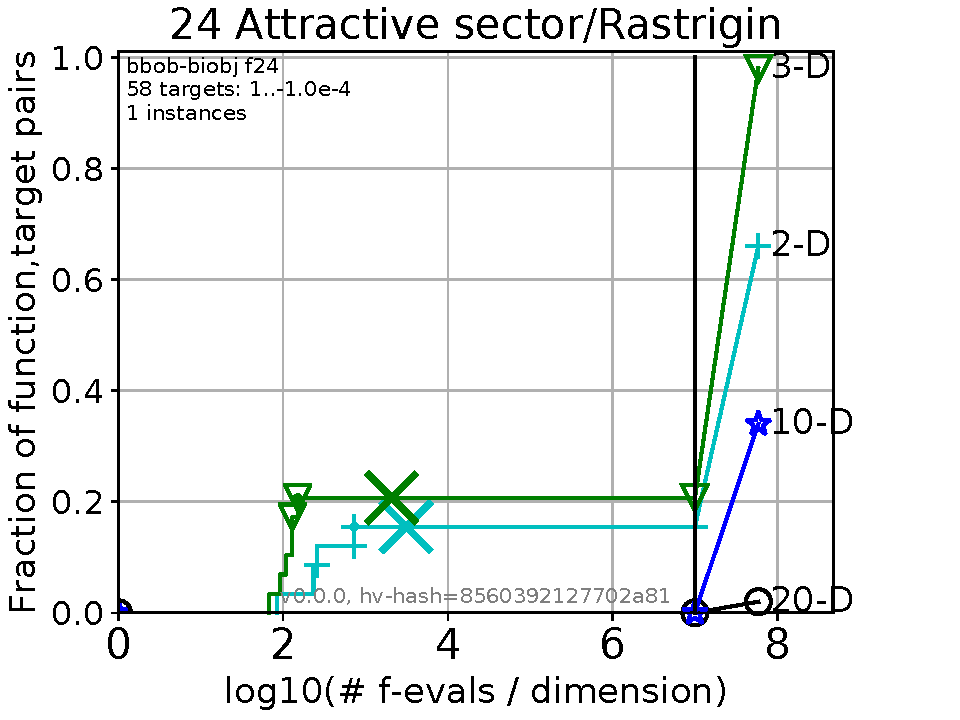
\includegraphics[width=0.25\textwidth]{pprldmany-single-functions/pprldmany_f024}\\
\includegraphics[width=0.25\textwidth]{pprldmany-single-functions/pprldmany_f025}&
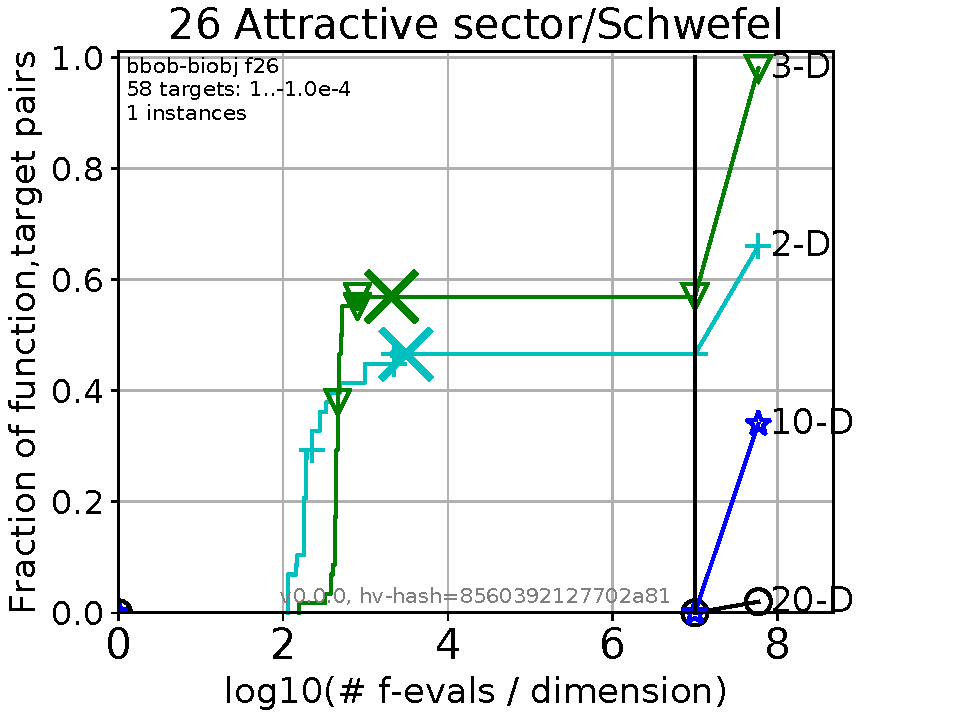
\includegraphics[width=0.25\textwidth]{pprldmany-single-functions/pprldmany_f026}&
\includegraphics[width=0.25\textwidth]{pprldmany-single-functions/pprldmany_f027}&
\includegraphics[width=0.25\textwidth]{pprldmany-single-functions/pprldmany_f028}\\
\includegraphics[width=0.25\textwidth]{pprldmany-single-functions/pprldmany_f029}&
\includegraphics[width=0.25\textwidth]{pprldmany-single-functions/pprldmany_f030}&
\includegraphics[width=0.25\textwidth]{pprldmany-single-functions/pprldmany_f031}&
\includegraphics[width=0.25\textwidth]{pprldmany-single-functions/pprldmany_f032}\\
\includegraphics[width=0.25\textwidth]{pprldmany-single-functions/pprldmany_f033}&
\includegraphics[width=0.25\textwidth]{pprldmany-single-functions/pprldmany_f034}&
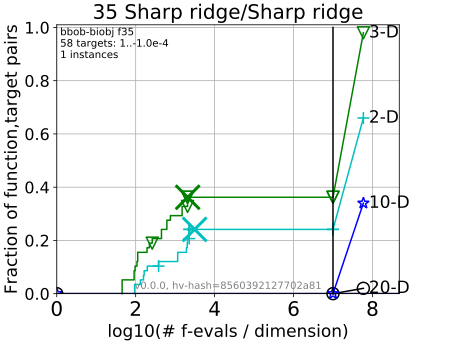
\includegraphics[width=0.25\textwidth]{pprldmany-single-functions/pprldmany_f035}&
\includegraphics[width=0.25\textwidth]{pprldmany-single-functions/pprldmany_f036}\\[-1.8ex]
\end{tabular}
 \caption{\label{fig:ECDFsingleTwo}
    Empirical cumulative distribution of simulated (bootstrapped) runtimes, 
    measured in number of objective function evaluations, divided by dimension 
    (FEvals/DIM) for the targets as given in Fig.~\ref{fig:ECDFsingleOne} 
    for functions 
    $f_{17}$ to $f_{36}$
    and all dimensions.
%
% Empirical cumulative distribution function (ECDF) per dimension for all 
% targets of each function as in Fig.~\ref{fig:ECDFsingleOne} but for $f_{17}$ till $f_{36}$.
 }
\end{figure*}
\begin{figure*}
\centering
\begin{tabular}{@{\hspace*{-0.018\textwidth}}l@{\hspace*{-0.02\textwidth}}l@{\hspace*{-0.02\textwidth}}l@{\hspace*{-0.02\textwidth}}l@{\hspace*{-0.02\textwidth}}l@{\hspace*{-0.02\textwidth}}}
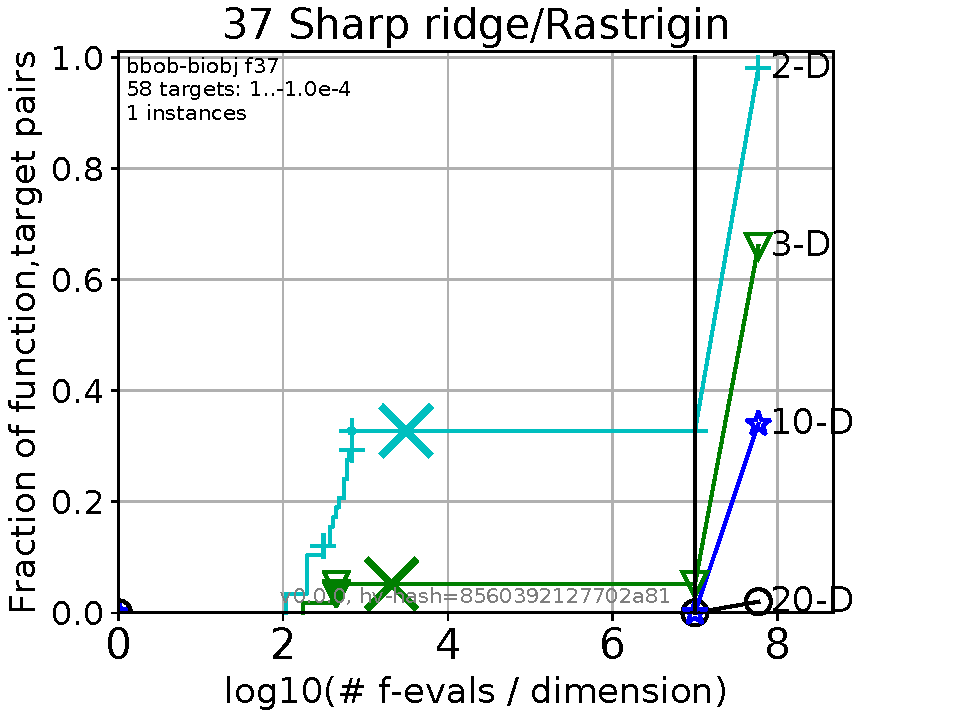
\includegraphics[width=0.25\textwidth]{pprldmany-single-functions/pprldmany_f037}&
\includegraphics[width=0.25\textwidth]{pprldmany-single-functions/pprldmany_f038}&
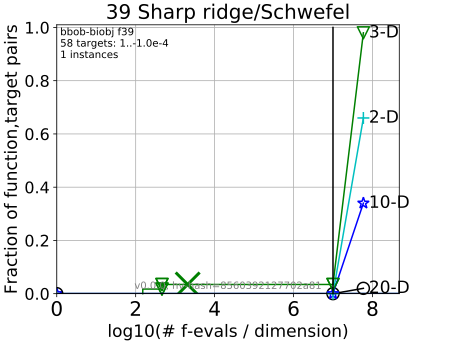
\includegraphics[width=0.25\textwidth]{pprldmany-single-functions/pprldmany_f039}&
\includegraphics[width=0.25\textwidth]{pprldmany-single-functions/pprldmany_f040}\\
\includegraphics[width=0.25\textwidth]{pprldmany-single-functions/pprldmany_f041}&
\includegraphics[width=0.25\textwidth]{pprldmany-single-functions/pprldmany_f042}&
\includegraphics[width=0.25\textwidth]{pprldmany-single-functions/pprldmany_f043}&
\includegraphics[width=0.25\textwidth]{pprldmany-single-functions/pprldmany_f044}\\
\includegraphics[width=0.25\textwidth]{pprldmany-single-functions/pprldmany_f045}&
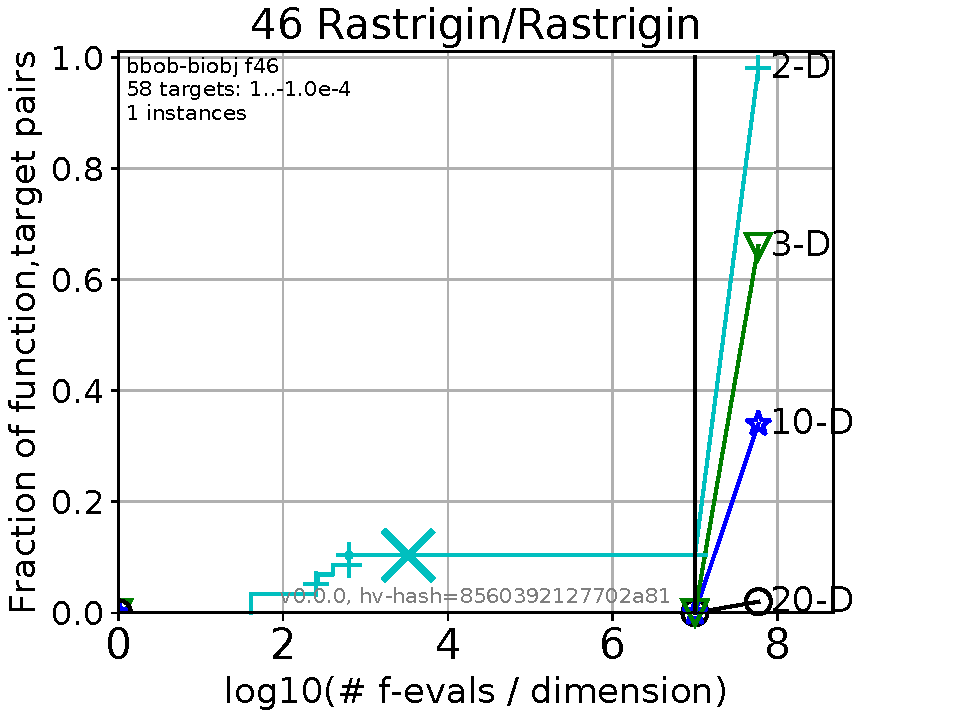
\includegraphics[width=0.25\textwidth]{pprldmany-single-functions/pprldmany_f046}&
\includegraphics[width=0.25\textwidth]{pprldmany-single-functions/pprldmany_f047}&
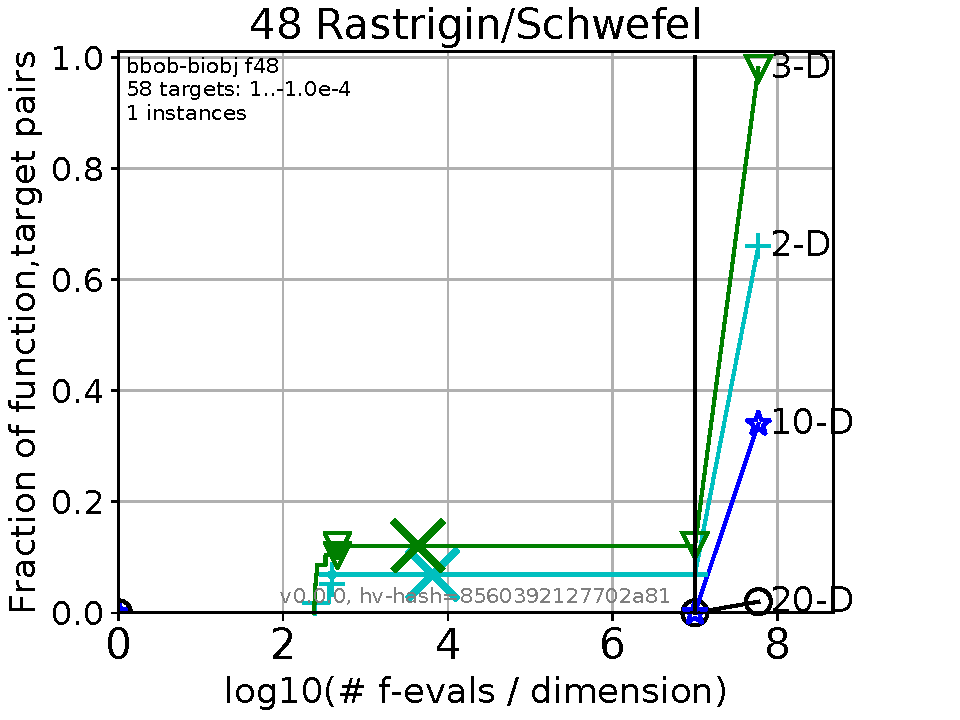
\includegraphics[width=0.25\textwidth]{pprldmany-single-functions/pprldmany_f048}\\
\includegraphics[width=0.25\textwidth]{pprldmany-single-functions/pprldmany_f049}&
\includegraphics[width=0.25\textwidth]{pprldmany-single-functions/pprldmany_f050}&
\includegraphics[width=0.25\textwidth]{pprldmany-single-functions/pprldmany_f051}&
\includegraphics[width=0.25\textwidth]{pprldmany-single-functions/pprldmany_f052}
\end{tabular}
\begin{tabular}{@{\hspace*{-0.018\textwidth}}l@{\hspace*{-0.02\textwidth}}l@{\hspace*{-0.02\textwidth}}l@{\hspace*{-0.02\textwidth}}l@{\hspace*{-0.02\textwidth}}}
\includegraphics[width=0.25\textwidth]{pprldmany-single-functions/pprldmany_f053}&
\includegraphics[width=0.25\textwidth]{pprldmany-single-functions/pprldmany_f054}&
\includegraphics[width=0.25\textwidth]{pprldmany-single-functions/pprldmany_f055}\\[-1.8ex]
\end{tabular}
 \caption{\label{fig:ECDFsingleThree}
    Empirical cumulative distribution of simulated (bootstrapped) runtimes, 
    measured in number of objective function evaluations, divided by dimension 
    (FEvals/DIM) for the targets as given in Fig.~\ref{fig:ECDFsingleOne} 
    for functions 
    $f_{37}$ to $f_{55}$
    and all dimensions. 
% Empirical cumulative distribution function (ECDF) per dimension for all targets of each function as in Fig.~\ref{fig:ECDFsingleOne} but for $f_{37}$ till $f_{55}$.
 }
\end{figure*}



%%%%%%%%%%%%%%%%%%%%%%%%%%%%%%%%%%%%%%%%%%%%%%%%%%%%%%%%%%%%%%%%%%%%%%%%%%%%%%%
%%%%%%%%%%%%%%%%%%%%%%%%%%%%%%%%%%%%%%%%%%%%%%%%%%%%%%%%%%%%%%%%%%%%%%%%%%%%%%%

% Empirical cumulative distribution functions (ECDFs) per function group.

%%%%%%%%%%%%%%%%%%%%%%%%%%%%%%%%%%%%%%%%%%%%%%%%%%%%%%%%%%%%%%%%%%%%%%%%%%%%%%%

\newcommand{\rot}[2][2.5]{
  \hspace*{-3.5\baselineskip}%
  \begin{rotate}{90}\hspace{#1em}#2
  \end{rotate}}
\begin{figure*}
\begin{tabular}{c@{\hspace*{-0.00\textwidth}}c@{\hspace*{-0.00\textwidth}}c@{\hspace*{-0.00\textwidth}}c}
separable-separable & separable-moderate & separable-ill-cond. & separable-multimodal\\
\includegraphics[width=0.24\textwidth]{pprldmany-single-functions/pprldmany_1-separable_1-separable} &
\includegraphics[width=0.24\textwidth]{pprldmany-single-functions/pprldmany_1-separable_2-moderate} &
\includegraphics[width=0.24\textwidth]{pprldmany-single-functions/pprldmany_1-separable_3-ill-conditioned} &
\includegraphics[width=0.24\textwidth]{pprldmany-single-functions/pprldmany_1-separable_4-multi-modal}\\
separable-weakstructure & moderate-moderate & moderate-ill-cond. & moderate-multimodal\\
\includegraphics[width=0.24\textwidth]{pprldmany-single-functions/pprldmany_1-separable_5-weakly-structured} &
\includegraphics[width=0.24\textwidth]{pprldmany-single-functions/pprldmany_2-moderate_2-moderate} &
\includegraphics[width=0.24\textwidth]{pprldmany-single-functions/pprldmany_2-moderate_3-ill-conditioned} &
\includegraphics[width=0.24\textwidth]{pprldmany-single-functions/pprldmany_2-moderate_4-multi-modal}\\
moderate-weakstructure & ill-cond.-ill-cond. & ill-cond.-multimodal & ill-cond.-weakstructure\\
\includegraphics[width=0.24\textwidth]{pprldmany-single-functions/pprldmany_2-moderate_5-weakly-structured} &
\includegraphics[width=0.24\textwidth]{pprldmany-single-functions/pprldmany_3-ill-conditioned_3-ill-conditioned} &
\includegraphics[width=0.24\textwidth]{pprldmany-single-functions/pprldmany_3-ill-conditioned_4-multi-modal} &
\includegraphics[width=0.24\textwidth]{pprldmany-single-functions/pprldmany_3-ill-conditioned_5-weakly-structured} \\
multimodal-multimodal & multimodal-weakstructure & weakstructure-weakstructure & all 55 functions\\
\includegraphics[width=0.24\textwidth]{pprldmany-single-functions/pprldmany_4-multi-modal_4-multi-modal} &
\includegraphics[width=0.24\textwidth]{pprldmany-single-functions/pprldmany_4-multi-modal_5-weakly-structured} &
\includegraphics[width=0.24\textwidth]{pprldmany-single-functions/pprldmany_5-weakly-structured_5-weakly-structured} &
\includegraphics[width=0.24\textwidth]{pprldmany-single-functions/pprldmany}
\vspace*{-0.5ex}
\end{tabular}
 \caption{\label{fig:ECDFsGroups}
 \bbobecdfcaptionallgroups{}
 }
\end{figure*}

%%%%%%%%%%%%%%%%%%%%%%%%%%%%%%%%%%%%%%%%%%%%%%%%%%%%%%%%%%%%%%%%%%%%%%%%%%%%%%%
%%%%%%%%%%%%%%%%%%%%%%%%%%%%%%%%%%%%%%%%%%%%%%%%%%%%%%%%%%%%%%%%%%%%%%%%%%%%%%%
 
% Table showing the average running time (aRT in number of function
% evaluations) to reach the given targets for functions $f_1$--$f_{55}$ for dimension 5.

%%%%%%%%%%%%%%%%%%%%%%%%%%%%%%%%%%%%%%%%%%%%%%%%%%%%%%%%%%%%%%%%%%%%%%%%%%%%%%%

\begin{table*}\tiny
\centering
\mbox{\begin{minipage}[t]{0.32\textwidth}\tiny
\centering
\pptableheader 

\input{\bbobdatapath\algfolder pptable_f001_05D} 

\input{\bbobdatapath\algfolder pptable_f002_05D}

\input{\bbobdatapath\algfolder pptable_f003_05D}

\input{\bbobdatapath\algfolder pptable_f004_05D}

\input{\bbobdatapath\algfolder pptable_f005_05D}

\input{\bbobdatapath\algfolder pptable_f006_05D}

\input{\bbobdatapath\algfolder pptable_f007_05D}

\input{\bbobdatapath\algfolder pptable_f008_05D}

\input{\bbobdatapath\algfolder pptable_f009_05D}

\input{\bbobdatapath\algfolder pptable_f010_05D}

\input{\bbobdatapath\algfolder pptable_f011_05D}

\input{\bbobdatapath\algfolder pptable_f012_05D}

\input{\bbobdatapath\algfolder pptable_f013_05D}

\input{\bbobdatapath\algfolder pptable_f014_05D}

\input{\bbobdatapath\algfolder pptable_f015_05D}

\input{\bbobdatapath\algfolder pptable_f016_05D}

\input{\bbobdatapath\algfolder pptable_f017_05D}

\input{\bbobdatapath\algfolder pptable_f018_05D}

\input{\bbobdatapath\algfolder pptable_f019_05D}

\pptablefooter

\end{minipage}
\hspace{0.002\textwidth}
\begin{minipage}[t]{0.32\textwidth}\tiny
\centering

\pptableheader 

\input{\bbobdatapath\algfolder pptable_f020_05D}

\input{\bbobdatapath\algfolder pptable_f021_05D}

\input{\bbobdatapath\algfolder pptable_f022_05D}

\input{\bbobdatapath\algfolder pptable_f023_05D}

\input{\bbobdatapath\algfolder pptable_f024_05D}

\input{\bbobdatapath\algfolder pptable_f025_05D}

\input{\bbobdatapath\algfolder pptable_f026_05D}

\input{\bbobdatapath\algfolder pptable_f027_05D}

\input{\bbobdatapath\algfolder pptable_f028_05D}

\input{\bbobdatapath\algfolder pptable_f029_05D}

\input{\bbobdatapath\algfolder pptable_f030_05D}

\input{\bbobdatapath\algfolder pptable_f031_05D}

\input{\bbobdatapath\algfolder pptable_f032_05D}

\input{\bbobdatapath\algfolder pptable_f033_05D}

\input{\bbobdatapath\algfolder pptable_f034_05D}

\input{\bbobdatapath\algfolder pptable_f035_05D}

\input{\bbobdatapath\algfolder pptable_f036_05D}

\input{\bbobdatapath\algfolder pptable_f037_05D}

\pptablefooter

\end{minipage}

\hspace{0.002\textwidth}
\begin{minipage}[t]{0.32\textwidth}\tiny
\centering

\pptableheader 

\input{\bbobdatapath\algfolder pptable_f038_05D}

\input{\bbobdatapath\algfolder pptable_f039_05D}

\input{\bbobdatapath\algfolder pptable_f040_05D}

\input{\bbobdatapath\algfolder pptable_f041_05D}

\input{\bbobdatapath\algfolder pptable_f042_05D}

\input{\bbobdatapath\algfolder pptable_f043_05D}

\input{\bbobdatapath\algfolder pptable_f044_05D}

\input{\bbobdatapath\algfolder pptable_f045_05D}

\input{\bbobdatapath\algfolder pptable_f046_05D}

\input{\bbobdatapath\algfolder pptable_f047_05D}

\input{\bbobdatapath\algfolder pptable_f048_05D}

\input{\bbobdatapath\algfolder pptable_f049_05D}

\input{\bbobdatapath\algfolder pptable_f050_05D}

\input{\bbobdatapath\algfolder pptable_f051_05D}

\input{\bbobdatapath\algfolder pptable_f052_05D}

\input{\bbobdatapath\algfolder pptable_f053_05D}

\input{\bbobdatapath\algfolder pptable_f054_05D}

\input{\bbobdatapath\algfolder pptable_f055_05D}

\pptablefooter

\end{minipage}}

 \caption[Table of aRTs]{\label{tab:aRTs5}\bbobpptablecaption{dimension $5$}
 }
\end{table*}
%sideways


%%%%%%%%%%%%%%%%%%%%%%%%%%%%%%%%%%%%%%%%%%%%%%%%%%%%%%%%%%%%%%%%%%%%%%%%%%%%%%%
%%%%%%%%%%%%%%%%%%%%%%%%%%%%%%%%%%%%%%%%%%%%%%%%%%%%%%%%%%%%%%%%%%%%%%%%%%%%%%%

% Table showing the average running time (aRT in number of function
% evaluations) to reach the given targets for functions $f_1$--$f_{55}$ for dimension 5.

%%%%%%%%%%%%%%%%%%%%%%%%%%%%%%%%%%%%%%%%%%%%%%%%%%%%%%%%%%%%%%%%%%%%%%%%%%%%%%%
\begin{table*}\tiny
\centering
\mbox{\begin{minipage}[t]{0.32\textwidth}\tiny
\centering
\pptableheader 

\input{\bbobdatapath\algfolder pptable_f001_20D} 

\input{\bbobdatapath\algfolder pptable_f002_20D}

\input{\bbobdatapath\algfolder pptable_f003_20D}

\input{\bbobdatapath\algfolder pptable_f004_20D}

\input{\bbobdatapath\algfolder pptable_f005_20D}

\input{\bbobdatapath\algfolder pptable_f006_20D}

\input{\bbobdatapath\algfolder pptable_f007_20D}

\input{\bbobdatapath\algfolder pptable_f008_20D}

\input{\bbobdatapath\algfolder pptable_f009_20D}

\input{\bbobdatapath\algfolder pptable_f010_20D}

\input{\bbobdatapath\algfolder pptable_f011_20D}

\input{\bbobdatapath\algfolder pptable_f012_20D}

\input{\bbobdatapath\algfolder pptable_f013_20D}

\input{\bbobdatapath\algfolder pptable_f014_20D}

\input{\bbobdatapath\algfolder pptable_f015_20D}

\input{\bbobdatapath\algfolder pptable_f016_20D}

\input{\bbobdatapath\algfolder pptable_f017_20D}

\input{\bbobdatapath\algfolder pptable_f018_20D}

\input{\bbobdatapath\algfolder pptable_f019_20D}

\pptablefooter

\end{minipage}
\hspace{0.002\textwidth}
\begin{minipage}[t]{0.32\textwidth}\tiny
\centering

\pptableheader 

\input{\bbobdatapath\algfolder pptable_f020_20D}

\input{\bbobdatapath\algfolder pptable_f021_20D}

\input{\bbobdatapath\algfolder pptable_f022_20D}

\input{\bbobdatapath\algfolder pptable_f023_20D}

\input{\bbobdatapath\algfolder pptable_f024_20D}

\input{\bbobdatapath\algfolder pptable_f025_20D}

\input{\bbobdatapath\algfolder pptable_f026_20D}

\input{\bbobdatapath\algfolder pptable_f027_20D}

\input{\bbobdatapath\algfolder pptable_f028_20D}

\input{\bbobdatapath\algfolder pptable_f029_20D}

\input{\bbobdatapath\algfolder pptable_f030_20D}

\input{\bbobdatapath\algfolder pptable_f031_20D}

\input{\bbobdatapath\algfolder pptable_f032_20D}

\input{\bbobdatapath\algfolder pptable_f033_20D}

\input{\bbobdatapath\algfolder pptable_f034_20D}

\input{\bbobdatapath\algfolder pptable_f035_20D}

\input{\bbobdatapath\algfolder pptable_f036_20D}

\input{\bbobdatapath\algfolder pptable_f037_20D}

\pptablefooter

\end{minipage}

\hspace{0.002\textwidth}
\begin{minipage}[t]{0.32\textwidth}\tiny
\centering

\pptableheader 

\input{\bbobdatapath\algfolder pptable_f038_20D}

\input{\bbobdatapath\algfolder pptable_f039_20D}

\input{\bbobdatapath\algfolder pptable_f040_20D}

\input{\bbobdatapath\algfolder pptable_f041_20D}

\input{\bbobdatapath\algfolder pptable_f042_20D}

\input{\bbobdatapath\algfolder pptable_f043_20D}

\input{\bbobdatapath\algfolder pptable_f044_20D}

\input{\bbobdatapath\algfolder pptable_f045_20D}

\input{\bbobdatapath\algfolder pptable_f046_20D}

\input{\bbobdatapath\algfolder pptable_f047_20D}

\input{\bbobdatapath\algfolder pptable_f048_20D}

\input{\bbobdatapath\algfolder pptable_f049_20D}

\input{\bbobdatapath\algfolder pptable_f050_20D}

\input{\bbobdatapath\algfolder pptable_f051_20D}

\input{\bbobdatapath\algfolder pptable_f052_20D}

\input{\bbobdatapath\algfolder pptable_f053_20D}

\input{\bbobdatapath\algfolder pptable_f054_20D}

\input{\bbobdatapath\algfolder pptable_f055_20D}

\pptablefooter

\end{minipage}}

 \caption[Table of aRTs]{\label{tab:aRTs20}\bbobpptablecaption{dimension $20$}
 }
\end{table*}

%%%%%%%%%%%%%%%%%%%%%%%%%%%%%%%%%%%%%%%%%%%%%%%%%%%%%%%%%%%%%%%%%%%%%%%%%%%%%%%
%\section{Discussion}  % and/or conclusions etc
%%%%%%%%%%%%%%%%%%%%%%%%%%%%%%%%%%%%%%%%%%%%%%%%%%%%%%%%%%%%%%%%%%%%%%%%%%%%%%%

%%%%%%%%%%%%%%%%%%%%%%%%%%%%%%%%%%%%%%%%%%%%%%%%%%%%%%%%%%%%%%%%%%%%%%%%%%%%%%%
% REFERENCES
%%%%%%%%%%%%%%%%%%%%%%%%%%%%%%%%%%%%%%%%%%%%%%%%%%%%%%%%%%%%%%%%%%%%%%%%%%%%%%%

\bibliographystyle{ACM-Reference-Format}
\bibliography{bbob}  % bbob.bib is the name of the Bibliography in this case

\clearpage % otherwise the last figure might be missing



\appendix
%%%%%%%%%%%%%%%%%%%%%%%%%%%%%%%%%%%%%%%%%%%%%%%%%%%%%%%%%%%%%%%%%%%%%%%%%%%%%%%
%%%%%%%%%%%%%%%%%%%%%%%%%%%%%%%%%%%%%%%%%%%%%%%%%%%%%%%%%%%%%%%%%%%%%%%%%%%%%%%

% Scaling of aRT with dimension

%%%%%%%%%%%%%%%%%%%%%%%%%%%%%%%%%%%%%%%%%%%%%%%%%%%%%%%%%%%%%%%%%%%%%%%%%%%%%%%
\begin{figure*}
\begin{tabular}{@{\hspace*{-0.0\textwidth}}l@{\hspace*{-0.0\textwidth}}l@{\hspace*{-0.0\textwidth}}l@{\hspace*{-0.0\textwidth}}l@{\hspace*{-0.0\textwidth}}l@{\hspace*{-0.0\textwidth}}}
\includegraphics[width=0.2\textwidth]{ppfigdim_f001}&
\includegraphics[width=0.2\textwidth]{ppfigdim_f002}&
\includegraphics[width=0.2\textwidth]{ppfigdim_f003}&
\includegraphics[width=0.2\textwidth]{ppfigdim_f004}&
\includegraphics[width=0.2\textwidth]{ppfigdim_f005}\\
\includegraphics[width=0.2\textwidth]{ppfigdim_f006}&
\includegraphics[width=0.2\textwidth]{ppfigdim_f007}&
\includegraphics[width=0.2\textwidth]{ppfigdim_f008}&
\includegraphics[width=0.2\textwidth]{ppfigdim_f009}&
\includegraphics[width=0.2\textwidth]{ppfigdim_f010}\\
\includegraphics[width=0.2\textwidth]{ppfigdim_f011}&
\includegraphics[width=0.2\textwidth]{ppfigdim_f012}&
\includegraphics[width=0.2\textwidth]{ppfigdim_f013}&
\includegraphics[width=0.2\textwidth]{ppfigdim_f014}&
\includegraphics[width=0.2\textwidth]{ppfigdim_f015}\\
\includegraphics[width=0.2\textwidth]{ppfigdim_f016}&
\includegraphics[width=0.2\textwidth]{ppfigdim_f017}&
\includegraphics[width=0.2\textwidth]{ppfigdim_f018}&
\includegraphics[width=0.2\textwidth]{ppfigdim_f019}&
\includegraphics[width=0.2\textwidth]{ppfigdim_f020}\\
\includegraphics[width=0.2\textwidth]{ppfigdim_f021}&
\includegraphics[width=0.2\textwidth]{ppfigdim_f022}&
\includegraphics[width=0.2\textwidth]{ppfigdim_f023}&
\includegraphics[width=0.2\textwidth]{ppfigdim_f024}&
\includegraphics[width=0.2\textwidth]{ppfigdim_f025}\\
\includegraphics[width=0.2\textwidth]{ppfigdim_f026}&
\includegraphics[width=0.2\textwidth]{ppfigdim_f027}&
\includegraphics[width=0.2\textwidth]{ppfigdim_f028}&
\includegraphics[width=0.2\textwidth]{ppfigdim_f029}&
\includegraphics[width=0.2\textwidth]{ppfigdim_f030}
\end{tabular}
\vspace{-3ex}
 \caption{\label{fig:aRTgraphs}
 \bbobppfigdimlegend{$f_1$ and $f_{30}$}
}
\end{figure*}


\begin{figure*}
\begin{tabular}{@{\hspace*{-0.0\textwidth}}l@{\hspace*{-0.0\textwidth}}l@{\hspace*{-0.0\textwidth}}l@{\hspace*{-0.0\textwidth}}l@{\hspace*{-0.0\textwidth}}l@{\hspace*{-0.0\textwidth}}}
\includegraphics[width=0.2\textwidth]{ppfigdim_f031}&
\includegraphics[width=0.2\textwidth]{ppfigdim_f032}&
\includegraphics[width=0.2\textwidth]{ppfigdim_f033}&
\includegraphics[width=0.2\textwidth]{ppfigdim_f034}&
\includegraphics[width=0.2\textwidth]{ppfigdim_f035}\\
\includegraphics[width=0.2\textwidth]{ppfigdim_f036}&
\includegraphics[width=0.2\textwidth]{ppfigdim_f037}&
\includegraphics[width=0.2\textwidth]{ppfigdim_f038}&
\includegraphics[width=0.2\textwidth]{ppfigdim_f039}&
\includegraphics[width=0.2\textwidth]{ppfigdim_f040}\\
\includegraphics[width=0.2\textwidth]{ppfigdim_f041}&
\includegraphics[width=0.2\textwidth]{ppfigdim_f042}&
\includegraphics[width=0.2\textwidth]{ppfigdim_f043}&
\includegraphics[width=0.2\textwidth]{ppfigdim_f044}&
\includegraphics[width=0.2\textwidth]{ppfigdim_f045}\\
\includegraphics[width=0.2\textwidth]{ppfigdim_f046}&
\includegraphics[width=0.2\textwidth]{ppfigdim_f047}&
\includegraphics[width=0.2\textwidth]{ppfigdim_f048}&
\includegraphics[width=0.2\textwidth]{ppfigdim_f049}&
\includegraphics[width=0.2\textwidth]{ppfigdim_f050}\\
\includegraphics[width=0.2\textwidth]{ppfigdim_f051}&
\includegraphics[width=0.2\textwidth]{ppfigdim_f052}&
\includegraphics[width=0.2\textwidth]{ppfigdim_f053}&
\includegraphics[width=0.2\textwidth]{ppfigdim_f054}&
\includegraphics[width=0.2\textwidth]{ppfigdim_f055}
\end{tabular}
\vspace{-3ex}
 \caption{\label{fig:aRTgraphsTwo}
 Runtime versus dimension as described in Fig.~\ref{fig:aRTgraphs}, here for functions $f_{31}$ to $f_{55}$.
 }
\end{figure*}

\end{document}
